This section presents benchmarks and tests that demonstrate 

%%%%%%%%%%%%%%%%%%%%%%%%%%%%%%%%%%%%%%%%%%%%%%%%%%%%%%%
\subsection{Deployment productivity}
%%%%%%%%%%%%%%%%%%%%%%%%%%%%%%%%%%%%%%%%%%%%%%%%%%%%%%%

\assign{Ben}

Benchmark the time to build and deploy a stack from scratch vs. with a build cache.

%%%%%%%%%%%%%%%%%%%%%%%%%%%%%%%%%%%%%%%%%%%%%%%%%%%%%%%
\subsection{Developer productivity}
%%%%%%%%%%%%%%%%%%%%%%%%%%%%%%%%%%%%%%%%%%%%%%%%%%%%%%%

\assign{Ben}

Squashfs deployment reduces configuration and compilation times compared to serving the same stack on a shared filesystem;

Benchmark configuration time and build time with the same stack stored in different locations:
\begin{itemize}
    \item mounted with squashfs-run
    \item in memory, i.e. \lstinline|/dev/shm|
    \item on scratch.
\end{itemize}

For the following:
\begin{itemize}
    \item simple hello world
    \item medium complexity application (Arbor)
    \item complex application, e.g. DLA-F
\end{itemize}

%%%%%%%%%%%%%%%%%%%%%%%%%%%%%%%%%%%%%%%%%%%%%%%%%%%%%%%
\subsection{Overheads}
%%%%%%%%%%%%%%%%%%%%%%%%%%%%%%%%%%%%%%%%%%%%%%%%%%%%%%%

\assign{Ben}

Quantify the memory overheads and affect on job startup time of mounting squashfs images on compute nodes at the start of SLURM jobs;

%%%%%%%%%%%%%%%%%%%%%%%%%%%%%%%%%%%%%%%%%%%%%%%%%%%%%%%
\subsection{Benchmarks and Applications}
%%%%%%%%%%%%%%%%%%%%%%%%%%%%%%%%%%%%%%%%%%%%%%%%%%%%%%%

\assign{JG (SPH-EXA), Antonk}

Micro-benchmarks and application benchmarks that demonstrate equivalent performance to applications compiled with CPE on the same system.

\todo{pick a couple of applications/micro-benchmarks to evaluate.}

benchmarks:
\begin{itemize}
    \item OSU benchmarks \assign{Ben Theo}
    \item SPH-EXA \assign{JG}
    \item \dots other?
\end{itemize}

% \subsubsection{SPH-EXA}
% \label{sec:sphexa}
%{{{ \section{NVIDIA A100 gpus}
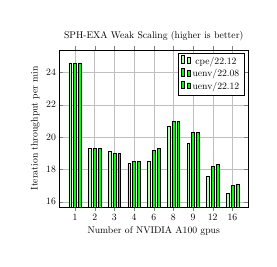
\begin{tikzpicture}[scale=0.35]
\label{fig:gpu-A100-best}
\begin{axis} [
    ybar, bar width = 3pt, symbolic x coords={1,2,3,4,6,8,9,12,16},
    xtick = data, grid=major, % legend pos=outer north east,
    xlabel=Number of NVIDIA A100 gpus, ylabel={Iteration throughput per min},
    title={SPH-EXA Weak Scaling (higher is better)},
]
% run-report-A100_64M-CPE_cpe2212.tbl
\addplot [fill=green!30!white] coordinates {
(1,24.6) (2,19.3) (3,19.1) (4,18.4) (6,18.5) (8,20.7) (9,19.6) (12,17.6) (16,16.5)
};
\addlegendentry{cpe/22.12}
% run-report-A100_64M-SQFS_cpe2208.tbl
\addplot [fill=green] coordinates {
(1,24.6) (2,19.3) (3,19.0) (4,18.5) (6,19.2) (8,21.0) (9,20.3) (12,18.2) (16,17.0)
};
\addlegendentry{uenv/22.08}
% run-report-A100_64M-SQFS_cpe2212.tbl
\addplot [fill=green] coordinates {
(1,24.6) (2,19.3) (3,19.0) (4,18.5) (6,19.3) (8,21.0) (9,20.3) (12,18.3) (16,17.1)
};
\addlegendentry{uenv/22.12}
\end{axis}
\end{tikzpicture}
% \captionof{figure}{your Caption}
%}}}
%{{{ \section{AMD MI200 gpus}
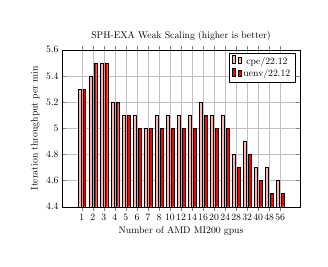
\begin{tikzpicture}[scale=0.35]
\label{fig:gpu-MI200-best}
\begin{axis} [
    ybar, bar width = 3pt,    
    x = 0.4cm, % space between bars
    symbolic x coords={1,2,3,4,5,6,7,8,10,12,14,16,20,24,28,32,40,48,56},
    xtick = data, grid=major, % legend pos=outer north east,
    xlabel=Number of AMD MI200 gpus,
    ylabel={Iteration throughput per min},
    title={SPH-EXA Weak Scaling (higher is better)},
]
% run-report-MI200_64M-CPE_cpe2212.tbl
\addplot [fill=red!30!white] coordinates {
(1,5.3) (2,5.4) (3,5.5) (4,5.2) (5,5.1) (6,5.1) (7,5.0) (8,5.1) (10,5.1) (12,5.1) (14,5.1) (16,5.2) (20,5.1) (24,5.1) (28,4.8) (32,4.9) (40,4.7) (48,4.7) (56,4.6)
};
\addlegendentry{cpe/22.12}
% run-report-MI200_64M-SQFS_cpe2212.tbl
\addplot [fill=red] coordinates {
(1,5.3) (2,5.5) (3,5.5) (4,5.2) (5,5.1) (6,5.0) (7,5.0) (8,5.0) (10,5.0) (12,5.0) (14,5.0) (16,5.1) (20,5.0) (24,5.0) (28,4.7) (32,4.8) (40,4.6) (48,4.5) (56,4.5)
};
\addlegendentry{uenv/22.12}
\end{axis} 
\end{tikzpicture}
%}}}
%{{{ results
The SPH-EXA\footnote{\url{https://github.com/unibas-dmi-hpc/SPH-EXA}} project is a multidisciplinary effort that looks to scale the Smoothed Particle Hydrodynamics (SPH) method to enable exascale hydrodynamics simulations for the fields of Cosmology and Astrophysics. 
Figure \ref{fig:gpu-A100-best} shows the performance obtained for the MPI+OpenMP+CUDA and MPI+OpenMP+HIP codes executing the Sedov--Taylor\footnote{\url{https://doi.org/10.48550/arxiv.2202.02840}} blast wave explosion test case with $400^3$ particles per gpu and $40$ time-steps.
The results show that the squashfs-based executables delivers competitive performance with that of the cpe based CPU executables on both NVIDIA A100 and AMD MI200 gpus.
%}}}

%%%%%%%%%%%%%%%%%%%%%%%%%%%%%%%%%%%%%%%%%%%%%%%%%%%%%%%
\subsection{Tools}
%%%%%%%%%%%%%%%%%%%%%%%%%%%%%%%%%%%%%%%%%%%%%%%%%%%%%%%

\assign{JG}

\begin{itemize}
    \item demonstrate DDT
    \item demonstrate a profiler?
\end{itemize}

%%%%%%%%%%%%%%%%%%%%%%%%%%%%%%%%%%%%%%%%%%%%%%%%%%%%%%%
\section{Future work}
%%%%%%%%%%%%%%%%%%%%%%%%%%%%%%%%%%%%%%%%%%%%%%%%%%%%%%%

We will discuss collaboration with HPE to provide Cray-MPICH and other HPE software packages via spack stacks, and how we plan to deliver software for the large Grace-Hopper scale out in the second half of 2023 at CSCS.

%%% Local Variables:
%%% TeX-master: "paper"
%%% End:
